\section{Konzept}
\label{sec:concept}

In den vorangegangenen Kapiteln wurde aufgezeigt, was die Dateiverwaltung der Schul-Cloud leisten muss und woran sie sich orientieren kann. Vom Partner des Bachelor-Projekts MINT-EC \footnote{Verein mathematisch-naturwissenschaftlicher Excellence-Center an Schulen e. V. (MINT-EC) - \url{https://www.mint-ec.de/}}  und dem Hasso-Plattner-Institut wurde eine Anforderungsspezifikation erstellt, an welcher sich das folgende Konzept der Dateiverwaltung orientiert (Abbildung \ref{fig:anforderungen}). Neben der Verwaltung von eigenen Dateien, sollen auch  jene im Kurs- bzw. Fächer- so wie Klassenkontext verteilbar sein. Dies soll dazu dienen, digitale Inhalte besser in den Unterricht einzubetten und (Haus)-Aufgaben mithilfe von anschaulichem Material zu gestalten. Somit sollen diese Dateien über eine einheitliche Schnittstelle durch die Backend-API sowie über das Web-Frontend in mehreren Kontexten verfügbar sein. Außerdem soll es für eine Schule möglich sein, eine bereits bestehende Dateiablage einzubinden. 

\begin{figure}[H]
	\centering
	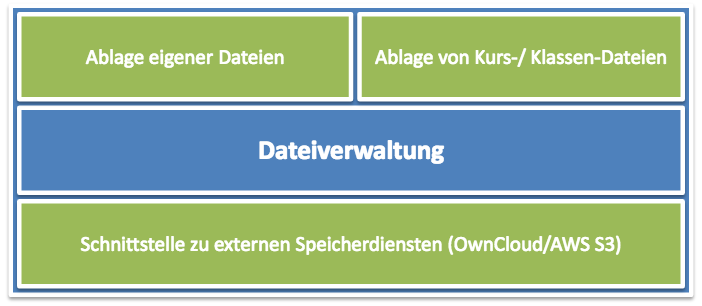
\includegraphics[width=0.8\linewidth]{images/AnforderungenDateiverwaltung}
	\caption[Caption for concept]{Grundanforderungen an die Dateiverwaltung der Schul-Cloud\footnotemark}
	\label{fig:anforderungen}
\end{figure}
\footnotetext{Martin Hense (Mint-EC - \url{https://www.mint-ec.de/})}


\subsection{Grundaufbau Dateiverwaltung}
\label{sec:basicaufbau}

Die grundlegende Struktur sieht vor, dass jede Schule seine eigene logische Einheit besitzt. Diese wird im folgenden \textit{Bucket} genant und leitet sich von der AWS S3-Nomenklatur ab (Abschnitt \ref{sec:awss3related}). Das dient zum einen der besseren Organisation innerhalb der Schul-Cloud, da Nutzer im Datenmodell zu einer Schule zusammengefasst werden. Außerdem folgt das Projekt dem Prinzip \textit{Privacy by Design} \footnote{Privacy by Design - \url{https://digitalcourage.de/blog/2015/was-ist-privacy-design} }. Damit wird sichergestellt, dass eine Schule von anderen modular abgekapselt wird. Somit ist von vornherein  eine Sicherheit der Dateien auf Schulebene gewährleistet. Diese Schul-Buckets können auf getrennten Servern liegen, so dass zum Beispiel eine Schule aus Niedersachsen auf eine eigene ownCloud zurückgreifen und eine Schule aus Hamburg einen S3-Provider benutzen kann. Das Prinzip des \textit{File Sharing} (Abschnitt \ref{sec:sharing_concept}) kann diese logische Abkapselung ein wenig aufbrechen, um Dateien auch über Schulebene hinaus teilbar zu machen. Eine Erweiterung von Buckets auf Landkreis - oder Bundeslandebene erscheint als weitere Option. Jedoch wird sich diese Arbeit auf die Einteilung in Schul-Buckets beschränken. Dieses Konzept ist aber ohne weiteres skalierbar auf größere Kontexte.  Die Abbildung \ref{fig:aufbau} zeigt im folgenden die weitere Unterteilung eines Buckets. Dieser wird in vier Teilkomponenten innerhalb der Schule  untergliedert. Wenn ein Bucket als einer Art Oberordner oder Root-Verzeichnis verstanden werden kann, dann sind diese Teilkomponenten schlichtweg Unterordner des Buckets. Zum einen gibt es den Ordner \textit{courses}, dieser enthält alle Dateien, welche zu Kursen bzw. Fächer gehören. Für eine bessere Unterteilung befinden sich hier sehr viele Unterordner, welche bloß die \textit{courseId} eines Schul-Cloud Kurses referenzieren. Dies dient der Verteilung aller Kurs-Dateien zu dem zugehörigen Kurs. Diese ID-Ordnernamen werden von Schul-Cloud Server versteckt und nicht im User Interface des  Clients angezeigt. So hat man aber zum Beispiel die Möglichkeit, über die \textit{courseId} alle Dateien eines Kurses zu erhalten. Auf diese haben nur Lehrer und Schüler des Kurses bzw. Faches Zugriff. Die Berechtigungsverwaltung übernimmt der Schul-Cloud Server und wird in der Implementierung (Abschnitt \ref{sec:permissionsimpl}) genauer beschrieben. \\

Ähnlich wie der \textit{courses} Unterordner gibt es den \textit{classes} und \textit{users} Unterordner. Beim ersten werden im gleichen Schema alle Dateien von Schul-Cloud Klassen verteilt, wieder referenziert über den jeweiligen ID-Unterordner. Zugriff haben hier nur Lehrer und Schüler der Klasse. Der \textit{users} Unterordner bildet die persönlichen Dateien eines jeden Nutzers der Schule, egal ob Lehrer, Schüler oder Administrator. Als Zusatz für schulübergreifende Dateien gibt es den Unterordner \textit{school}. Schreibrechte hat hier nur der Administrator der Schule, zugreifen kann jedoch jeder Nutzer der Schule. Natürlich kann es nun vorkommen, dass eine Schule bereits eine ausgeprägte Dateistruktur besitzt und der Grundaufbau mit den vier Unterkomponenten nicht abbildbar sein könnte. Hier muss der Schul-Cloud Server dafür sorgen, dass diese Dateien trotzdem über die Schul-Cloud zugänglich sind. Eine Möglichkeit wäre es, dass die gesamte Struktur zu Beginn in den \textit{schools} Ordner gelegt wird und diese von dahin auf die jeweiligen Kontexte verlegt werden.

\begin{figure}[H]
	\centering
	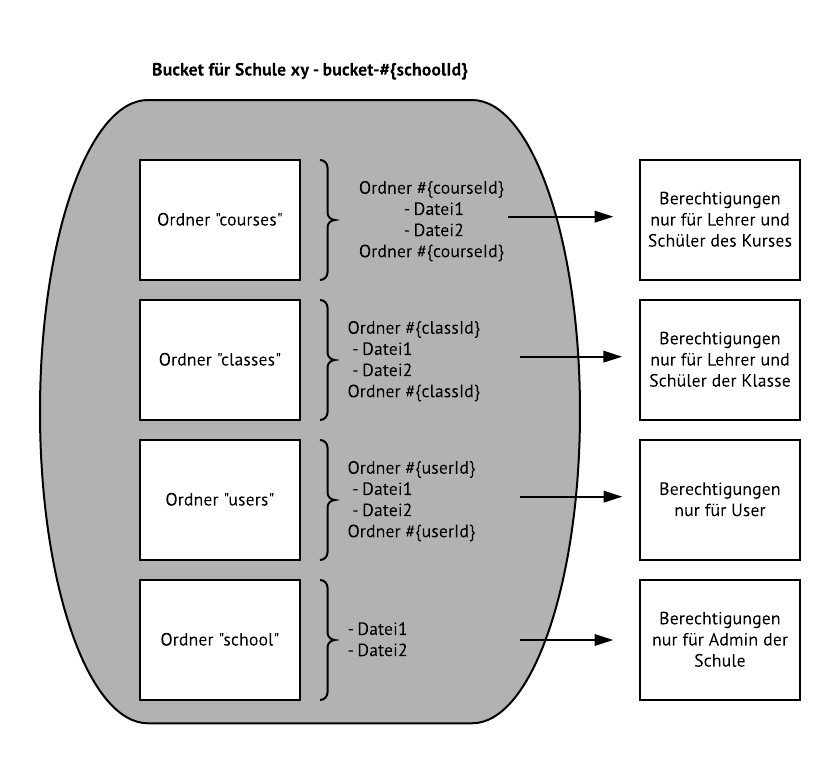
\includegraphics[width=0.8\linewidth]{images/AufbauDateiverwaltung}
	\caption[Caption for concept]{Grundaufbau eines Schul-Buckets}
	\label{fig:aufbau}
\end{figure}

\subsection{Architektur verteilter Provider}
\label{sec:strategypatternconcept}

Die Schul-Cloud stellt während der Pilotphase zwar nur eine S3-Instanz \footnote{Technischer Bericht der Schul-Cloud, Seite 39 \cite{paper:technischerbericht}}, worauf die Buckets der Pilotschulen liegen. Trotzdem soll es die Architektur der Dateiverwaltung möglich machen, Buckets auch auf mehrere Server zu verteilen. Dafür macht sich der Server das Strategy-Pattern \footnote{Strategy-Pattern - \url{https://de.wikipedia.org/wiki/Strategie_(Entwurfsmuster)}} zu Nutze. Dieses sieht vor, dass eine abstrakte Strategie die Schnittstellen vorgibt und mehrere Strategien diese implementieren. In Form dieser können so Anbindungen an verschiedene Typen von File Storage Providern erstellt werden. In der Implementierung wird eine solche Strategie am Beispiel von AWS S3 (Abschnitt \ref{sec:awss3impl}) geschildert. Abbildung \ref{fig:strategy} zeigt die Verteilung der verschiedenen File Storage Strategien. So ist es möglich, über den Schul-Kontext, der die Art des Provider bestimmt, die richtige Strategie zu bestimmen und auf die Schuldateien zugreifen zu können. Diese Aufteilung macht die Verteilung von Buckets auf mehrere Server ausführbar. So kann ein Bucket auf einer S3-Instanz liegen und mittels S3-Strategie darauf zugegriffen werden, sowie eine ownCloud-Instanz durch die ownCloud-Strategie auf einem anderen Server. Zwar ähnelt die genannte Struktur sehr dem S3-Ansatz, er lässt sich jedoch auch auf andere Typen einsetzen. Ein Bucket im ownCloud-Kontext kann hierbei ein normaler ownCloud-Ordner sein, der durch bestimmte Sicherheitsvorkehrungen und Einstellungen nur für den Schul-Administrator zugänglich ist.

\begin{figure}[H]
	\centering
	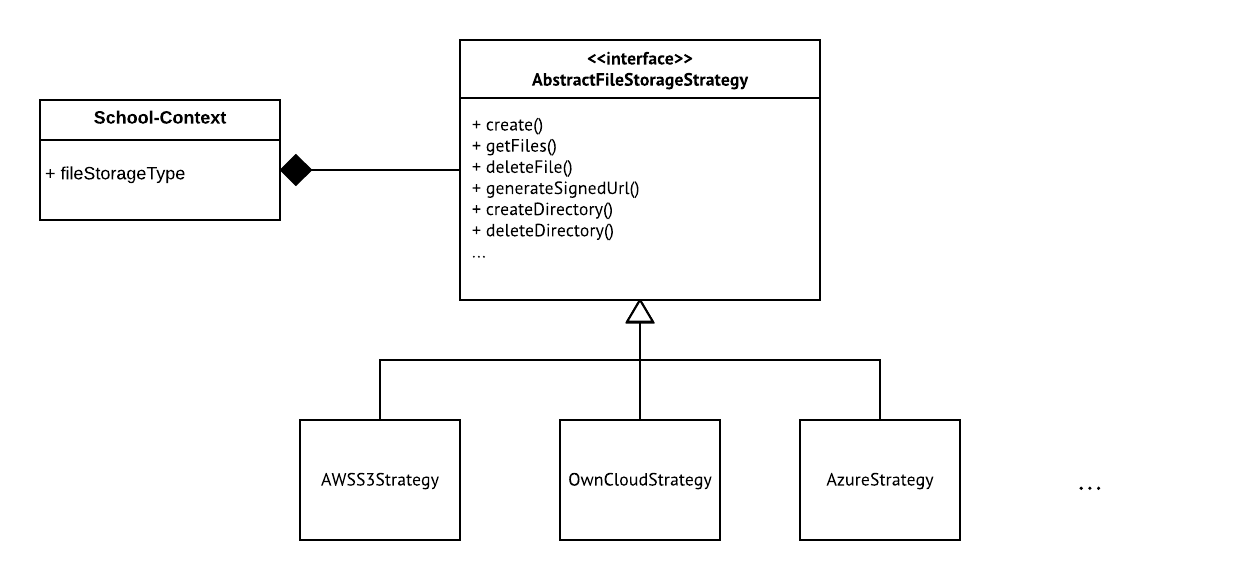
\includegraphics[width=1\linewidth]{images/strategypattern}
	\caption[Caption for concept]{Verteilung der Schul-Buckets mithilfe des Strategy-Patterns}
	\label{fig:strategy}
\end{figure}

\subsection{Interaktion verschiedener Schul-Cloud Komponenten}
\label{sec:interactionconcept}

Im Folgenden wird die Interaktion der verschiedenen Schul-Cloud Komponenten mithilfe von Beispielen beschrieben. Es wird stets von drei Rollen der Kommunikation geredet. Zum einen sorgt der \textit{Client} für die Nutzeraktion und steht somit für das Schul-Cloud Frontend, aber auch für eine mobile App. Der \textit{Server} meint den Schul-Cloud Server und dient als einer Art Proxy zu den verschiedenen File-Storage Providern. Dieser wird im Folgenden als \textit{Provider} bezeichnet. Als erstes Beispiel soll das Holen der persönlichen Dateien dienen. Abbildung \ref{fig:interacton_getFiles} zeigt die Interaktion der drei Komponenten. Der Client beginnt hierbei mit einem GET-HTTP-Request an die \textit{/fileStorage/} - Route vom Server. Um Dateien für einen bestimmten Kontext zu bekommen, muss im Query-Parameter \textit{path} der richtige Pfad mitgegeben werden. Für die persönlichen Dateien des Nutzers mit der ID \textit{123} ist dies \textit{users/123}. Man sieht hierbei die Rückführung auf den Grundaufbau der Dateiverwaltung. Die persönlichen Dateien eines jeden Schul-Cloud Nutzers werden im \textit{users} Unterordner der zugehörigen Schule gespeichert. Der ID-Ordner referenziert hier die Dateien des gesuchten Nutzers mit der ID \textit{123}. Dies muss eine valide Nutzer-ID sein, welche in der Schul-Cloud Datenbank gespeichert wird. Der Server kümmert sich nun um die Berechtigung, in dem er zum einen prüft, ob der im Client angemeldete Nutzer auch auf den Pfad zugreifen darf. Im Detail wird dies noch im Abschnitt \ref{sec:permissionsimpl}. beschrieben. Der Server ermittelt die Schule des Nutzers und fragt dann beim richtigen Provider die gesuchten Dateien für den gegebenen Pfad an. Dieser gibt dann die Datei-Objekte aus, welche dann über den Server zum Client ausgegeben werden. Man sieht hier sehr gut, dass der Schul-Cloud Server eine verwaltende Rolle einnimmt, ohne die Dateien tatsächlich physisch zu speichern. Er sorgt vielmehr für die Verteilung der Requests an die richtigen File Storage Provider. Dafür nutzt er das zuvor dargestellte Strategy-Pattern, um für eine Schule den richtigen Bucket zu finden.

\begin{figure}[H]
	\centering
	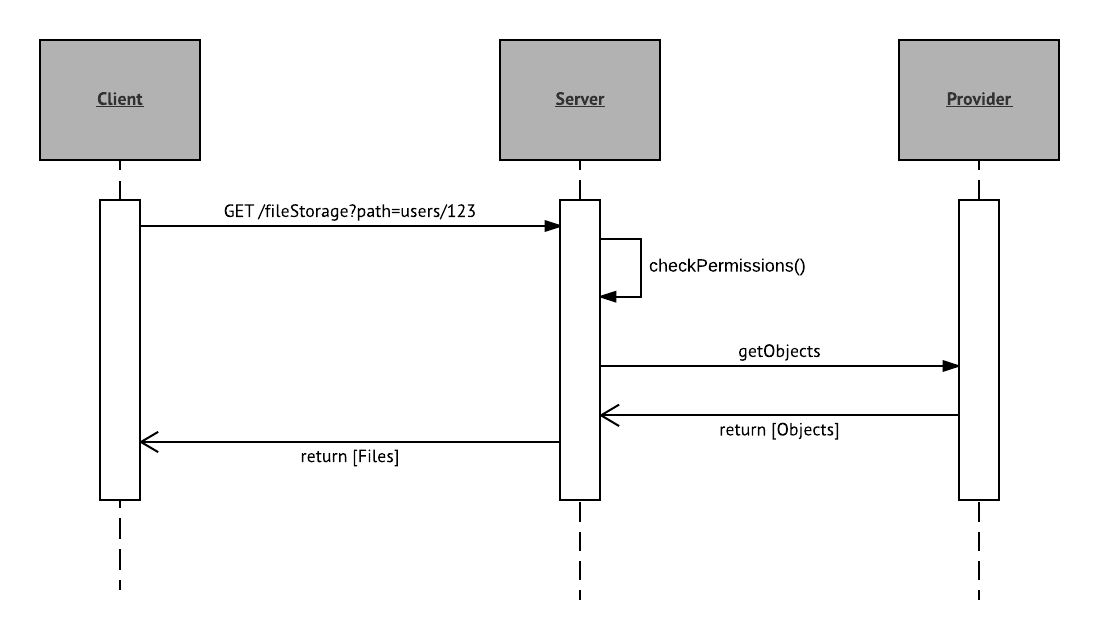
\includegraphics[width=1\linewidth]{images/fileumlsequence}
	\caption[Caption for concept]{Interaktion zwischen Client, Server und File Storage Provider  beim Holen von persönlichen Dateien}
	\label{fig:interacton_getFiles}
\end{figure}

Neben dieser einfachen dreigeteilten Interaktion zwischen Client, Server und Provider werden Upload und Download von Dateien direkt zwischen Client und Provider gehandhabt. Das hat den Grund, dass die Übertragung großer Datenmengen bei Dateien im Gigabyte - Bereich nicht über den Server laufen sollen. Abbildung \ref{fig:interaction_upload} zeigt dies anhand des Uploads einer Datei. Der Server fragt beim Provider nun eine Upload-URL an, auf welche der Client dann die Datei \textit{example.jpg} hochladen kann. Der Query-Parameter \textit{action} teilt mit, um welchen Typ von URL es sich handelt, im Falle von \textit{putObject} beim Upload einer Datei. Der Server prüft wieder die Berechtigungen des Clients und sendet dann die URL an den Client zusammen mit wichtigen Meta-Daten der Datei zurück. Diese soll der Client zusammen mit der Datei zum Provider laden, damit der Server später mehr Informationen über die Datei hat, zum Beispiel die Referenzierung eines Vorschaubilds.

\begin{figure}[H]
	\centering
	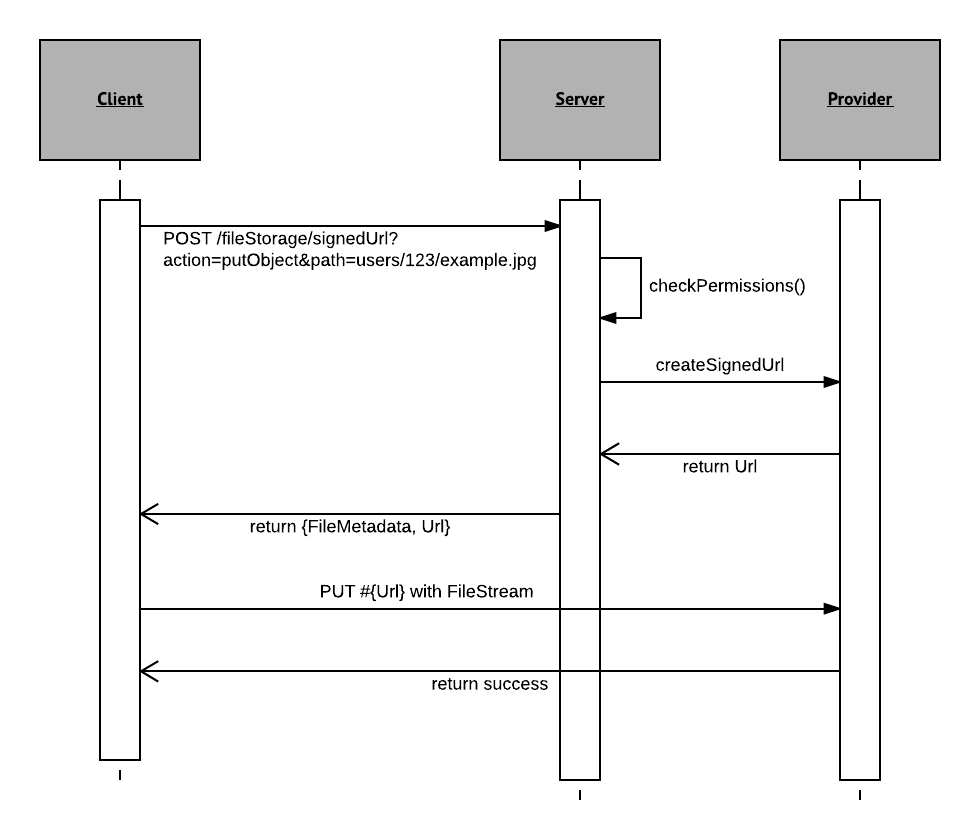
\includegraphics[width=1\linewidth]{images/fileuploadumlsequence}
	\caption[Caption for concept]{Interaktion zwischen Client, Server und File Storage Provider beim Upload einer Datei}
	\label{fig:interaction_upload}
\end{figure}


\subsection{Teilen von Dateien}
\label{sec:sharing_concept}

Zwar gibt der Aufbau der Dateiverwaltung eine klare Aufteilung zwischen Schul-, Kurs-, Fach - und Klassenkontexten vor, es soll jedoch trotzdem möglich sein, Dateien mit anderen Nutzern zu teilen. Das ist vor allem dann von Vorteil, wenn ein Lehrer eine persönliche Datei in seinem Unterricht direkt benutzen möchte. Zwar könnte der Lehrer dann die Datei in den jeweiligen Kursordner hochladen bzw. direkt im Unterrichtsmodus des Clients hochladen; welcher im Abschnitt \ref{sec:client} beschrieben wird; manchmal möchte der Lehrer trotzdem seine eigenen Dateien bei sich behalten und die Freigabe selbst steuern können. Ein weiteres Beispiel wäre es, wenn ein Schüler eine private Datei mit anderem teilen möchte, ohne sie im Kurskontext verfügbar zu machen. Somit muss es möglich sein, im Schul-Cloud Client einen Zugriffslink zu generieren. Dieses Prinzip findet auch bei ownCloud sowie Dropbox Einsatz und ist ein beliebter Weg, eigene Dateien schnell mit mehreren Personen zu  teilen. Abbildung \ref{fig:filesharinggeneration} zeigt den Prozess zur Generierung eines solchen Links für eine Datei. Der Client fordert die Freischaltung für das Teilen der Datei beim Server an. Dieser besteht intern aus dem eigentlichen File-Service und aus dem Link-Service, welcher als URL  Shortener \footnote{Kurz-URL-Dienst - \url{https://de.wikipedia.org/wiki/Kurz-URL-Dienst}} auftritt. Dieser dient dazu, den langen Link zu einer Schul-Cloud Datei etwas zu verkürzen und leichter teilbar zu machen. Nachdem der File-Service das Teilen freigegeben hat, fragt der Client einen solchen Shortlink an und gibt diesen im User Interface an. Dieser Prozess ist bekannt aus bereits bestehenden File Storage Providern.

\begin{figure}[H]
	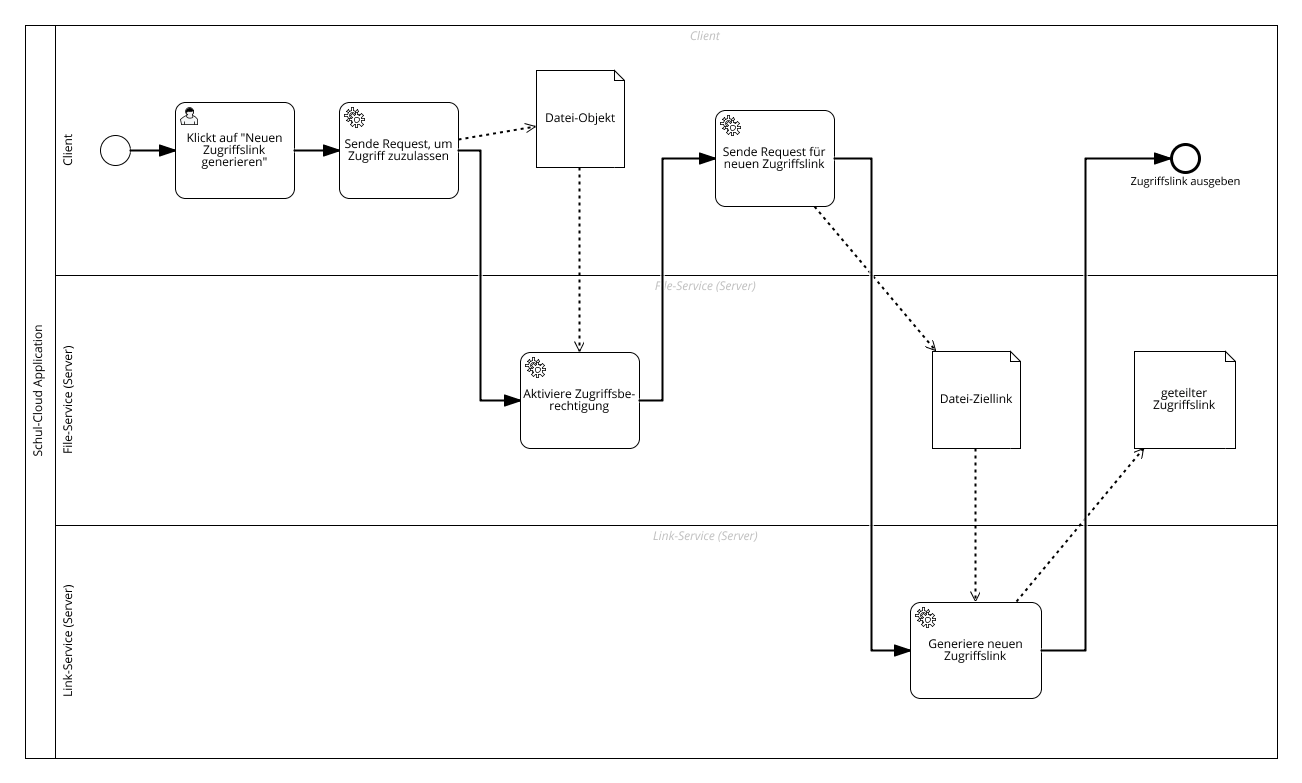
\includegraphics[width=1\linewidth]{images/filesharinggeneration}
	\caption[Caption for concept]{Generierung eines Zugriffslinks}
	\centering
	\label{fig:filesharinggeneration}
\end{figure}

Diesen Link kann der Besitzer der Datei nun an andere Schul-Cloud Nutzer weiterleiten. Den daraus resultierenden Zugriff ist in Abbildung \ref{fig:filesharingusing} modelliert. Der Client öffnet den Link und fragt zuerst beim Server an, ob die Sharing-Funktion für die Datei überhaupt freigeschaltet ist. Ist dies nicht freigegeben, erhält der Client einen Fehler. Im anderen Falle wird im Server gespeichert, welcher Nutzer auf die Datei zugreifen möchte, um den Prozess später zu beschleunigen und redundante Prüfungen zu verhindern. Außerdem können so für den Nutzer freigegebene Dateien zusammen aufgelistet werden, wie es Dropbox beispielsweise tut. Anschließend wird eine Anfrage auf die tatsächliche Datei über den Server an den Storage Provider gestellt und diese zurück an den Client gesendet. Dieser Teil des Prozesses ist sehr vereinfacht dargestellt, tatsächlich muss für das Holen der tatsächlichen Datei zunächst eine Zugriffs-URL, wie in Abschnitt \ref{sec:interactionconcept} beschrieben, generiert werden und an den Client geliefert werden.

\begin{figure}[H]
	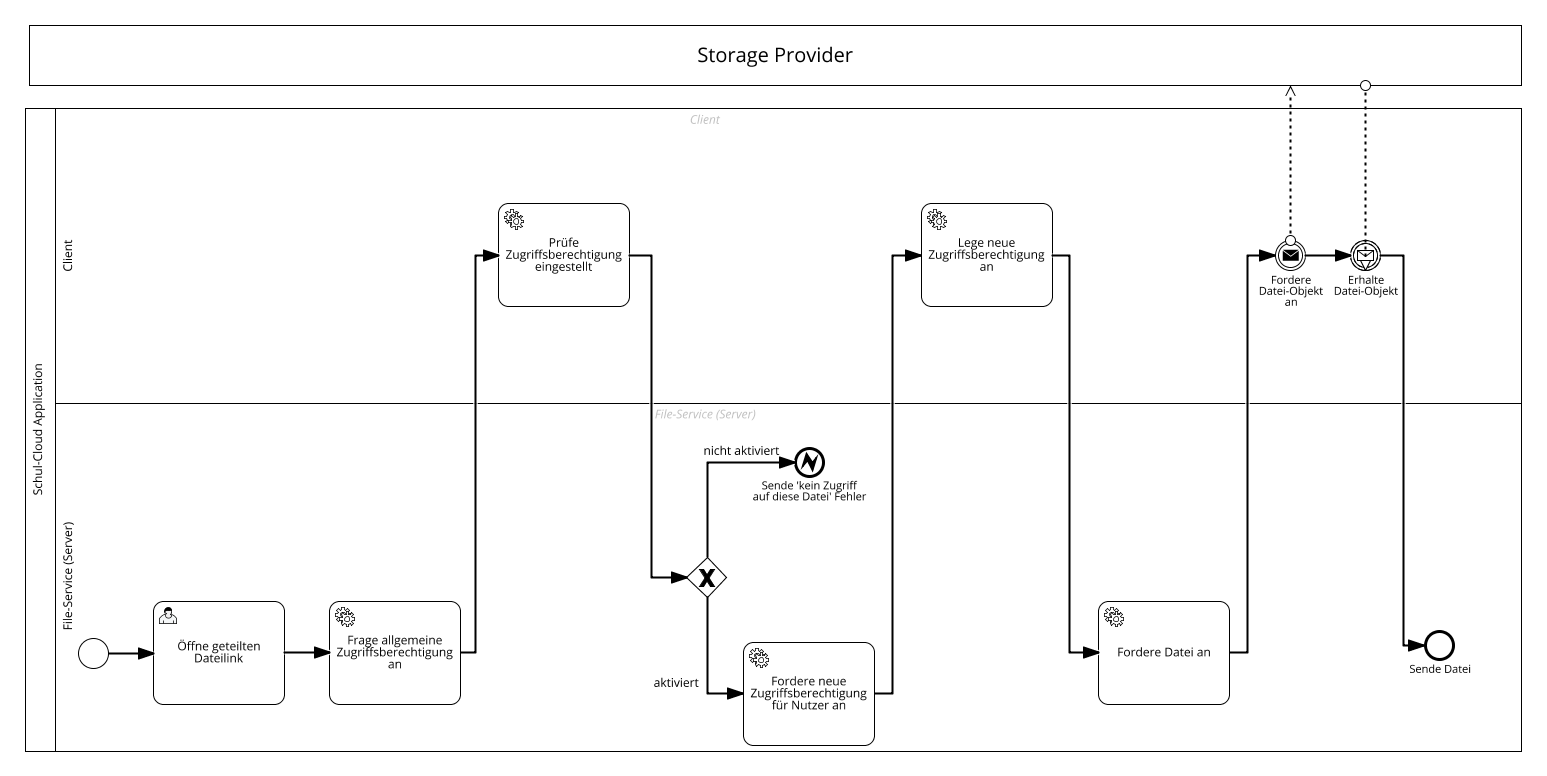
\includegraphics[width=1\linewidth]{images/filesharingusing}
	\caption[Caption for concept]{Zugriff auf eine geteilte Datei}
	\centering
	\label{fig:filesharingusing}
\end{figure}


\clearpage
